\chapter{Desarrollo}
\label{chapter:Desarrollo}

En esta parte de la memoria se detallarán los pasos seguidos durante el desarrollo y la aplicación de los algoritmos de \textit{Machine Learning} sobre los datos utilizados. Asimismo, se entrará en profundidad en los datos utilizados y como se han preprocesado para su posterior aplicación en los algoritmos.

Generalmente, la mayor parte del tiempo de un proyecto de \textit{Data Science} se invierte en la extracción y preprocesado de los mismos hasta que tengan la suficiente calidad como para arrojar resultados decentes tras aplicar los algoritmos. Para este proyecto esto ha sido el caso, la mayor parte de los esfuerzos han sido en la comprensión de los datos y como hacer frente (tanto por tiempo como por tamaño) a los datos disponibles.

Tanto el preprocesado como la aplicación de los algoritmos de \textit{Machine Learning} se ha realizado utilizando el lenguaje de programación \textit{Python} en su versión 3.6 y la exploración y análisis de los datos se han realizado en \textit{Jupyter Notebooks} para facilitar la visualización de los datos y las acciones tomadas. Todo se ha realizado en una máquina remota proporcionada por la UOC con 10 núcleos y 64gb de memoria RAM.
\newpage

\section{Datos utilizados}

Para este proyecto se va a utilizar un \textit{dataset} con información de las conexiones entre dispositivos IOT, mediante el análisis de los paquetes obtenidos por un analizador de paquetes o \textit{sniffer} el cual se trata de un software que permite observar y recopilar las acciones que desarrollan dentro de una red \cite{sniffer}. Utilizando los datos recopilados por este software se preprocesarán de modo que se pueda extraer la información y posteriormente transformarla y crear nuevas variables.

Los datos iniciales se trataban de unos datos ya preprocesados inicialmente con la información de las anomalías (únicamente anomalías) que se habían recopilado en un espacio de tiempo de dos meses. En este caso los datos solo contaban con tráfico ilegitimo, por lo que no se podía hacer una detección de anomalías como tal.

Posteriormente, se proporcionaron los datos en bruto en un fichero de extensión \textit{pcap} resultante del \textit{sniffer} mencionado anteriormente. Este fichero contiene información de las distintas capas en las que se almacenan los datos, siendo las de más interés las capas \textit{TCP} e \textit{IP}.

\begin{itemize}
    \item \textit{Transmission Control Protocol}: originario de los años 70/80 se trata de un protocolo para la transmisión de paquetes en conexiones \textit{host} a \textit{host} en redes \cite{postel1981transmission}
    \item \textit{Internet Protocol}: protocolo que permite la transmisión de datos de origen a destino donde el origen y el destino son direcciones de longitud fija y proporciona los medios para la división y reagrupación de grandes datos en grupos más pequeños \cite{postel1981internet} 
\end{itemize}

Sobre estas capas se obtiene la información disponible al más bajo nivel y posteriormente se generarán nuevas variables en base a los datos obtenidos. Siendo los datos de la capa TCP los siguientes:

\begin{itemize}
    \item Puerto de origen: indica el puerto de origen utilizado para realizar la conexión desde la IP de origen
    \item Puerto de destino: indica el puerto de destino utilizado en la conexión entre \textit{hosts}
\end{itemize}
\newpage

Los datos obtenidos de la capa IP:
\begin{itemize}
    \item IP de origen: dirección con longitud fija del origen de la conexión
    \item IP de destino: dirección con longitud fija del destino de la conexión
    \item \textit{Length}: longitud/tamaño de los paquetes enviados durante la conexión
\end{itemize}

\begin{figure}[H]
    \centering
    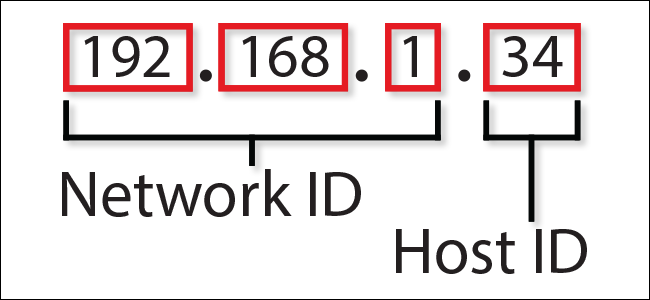
\includegraphics[width=6cm]{figs/ip.png}
    \caption{Ejemplo de dirección IPv4}
    \label{fig:wireshark}
\end{figure}

Otros datos:

\begin{itemize}
    \item \textit{Payload}: contenido de los datos transmitidos, pudiendo ser texto, imágenes o comandos a ejecutar en el \textit{host} de destino, con posibilidad de estar cifrado
    \item \textit{Timestamp}: marca tiempo que indica en que momento se realizó la conexión
\end{itemize}

Un ejemplo más visual de los datos a bajo nivel se puede realizar utilizando la herramienta \textit{Open Source, Wireshark}, fundamental a la hora de entender como están distribuidos los datos en las capas.

\begin{figure}[H]
    \centering
    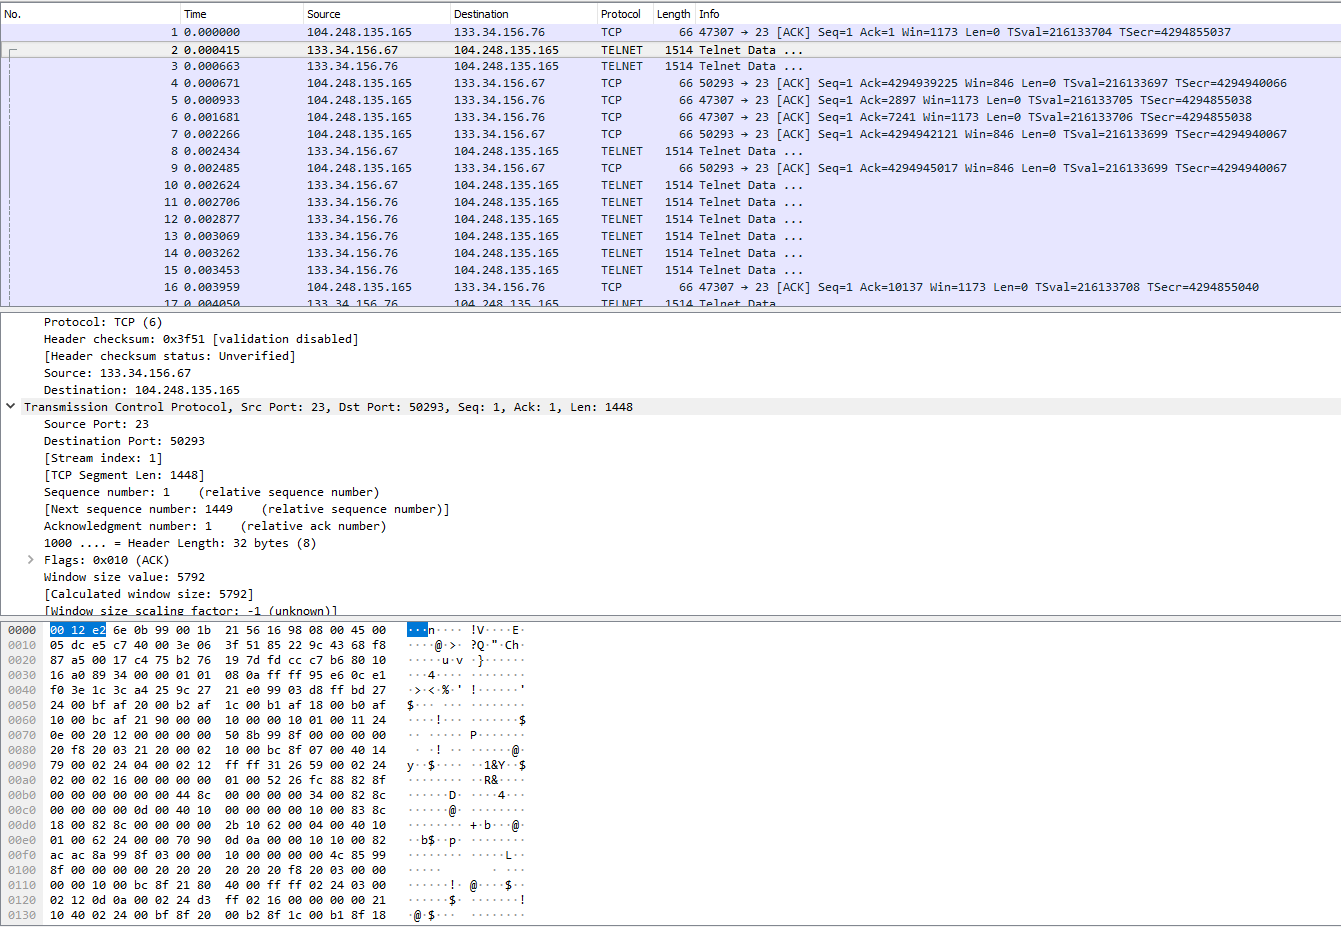
\includegraphics[width=15cm]{figs/wireshark.PNG}
    \caption{Ejemplo de datos pcap en Wireshark}
    \label{fig:wireshark}
\end{figure}

El \textit{Timestamp} puede indicar que el problema debería de tratarse como una serie temporal y generar variables en base a ésta característica.

Los datos provienen de la recolección de información realizada el dos de Febrero de 2019, contando tanto con tráfico legítimo como ilegítimo, sin embargo no existe clasificación de los datos, por lo que estamos tratando de un problema de carácter no supervisado, por lo que se utilizarán técnicas como las descritas en el capítulo \ref{chapter:Estado del Arte} de aprendizaje no supervisado.

\newpage